\documentclass{article}
\title{Report on workshop with FMCW radar}
\author{Pavlo Tokariev\\Inria, I3S, Université Côte d'Azur, Sophia Antipolis}
\date{\today}

\usepackage{amssymb, amsmath}
\usepackage{siunitx}
\usepackage{tikz}
\usetikzlibrary {shapes.geometric}
\usepackage{pgfplots}
\usepackage{hyperref}

\begin{document}
\maketitle

\section{Introduction}
\label{sec:introduction}

In this report we discuss a workshop that was conducted in the course "Introduction to Scientific Research".
As part of the effort to document the experiment to make it reproducible, we describe the parameters of the experiment, data processing steps and physical principles that explain the experiment.
We also discuss objectives and general structure of the workshop.

The workshop is centered about a radar experiment and analysis of the radar output data with the objective to recognize an object opposite of a radar.

The workshop can be divided it into two parts: the first is the radar setup, launch of measurements and data retrieval, and the second is the data processing.
In the measurement part, we installed the radar in a relatively open area, with no visible obstacle on the line of sight between the radar and the object.
After making a series of pulses and collecting the received reflected waves, we place a solid object in front of the radar.
We note the distance between the radar and the object, and repeat the measurements.

The role of data processing is then to compute distance information about the surrounding objects from both of the measurements.
By calculating difference between the two, we can obtain information on the environment change, or in other words, we can clearly identify a new body and distance to it.
This body should be found exactly where we placed the object before the second round of measurements.

The objective\footnote{The objectives are inferred and may be incorrect.} of the workshop is to show the complexity of modern scientific work.
In the span of 3 hours we covered experiment materials installation and the importance of a proper method that minimizes errors, discussed the main principle of the radar and the logic of its output processing in order to calculate the distance data.
This covers at least the general ideas on experiment organization, some elements of physics and math, and computer tools on numerical calculations.

The report is divided into several sections.
Section~\ref{sec:setting} presents the experiment setting, including physical placement of the hardware, parameters and type of the radar, as well as its general structure.
Section~\ref{sec:radar-working-principle} explains the working principle of the radar.
Section~\ref{sec:data-post-processing} describes the complete procedure to obtain distance to an object.
Section~\ref{sec:criticism} discusses ways to improve the experiment by describing factors that could lead to errors.
Section~\ref{sec:conclusion} concludes the report.


\section{Radar setting}
\label{sec:setting}

\subsection{Placement}
\label{subsec:placement}
\begin{figure}[h]
    \centering
    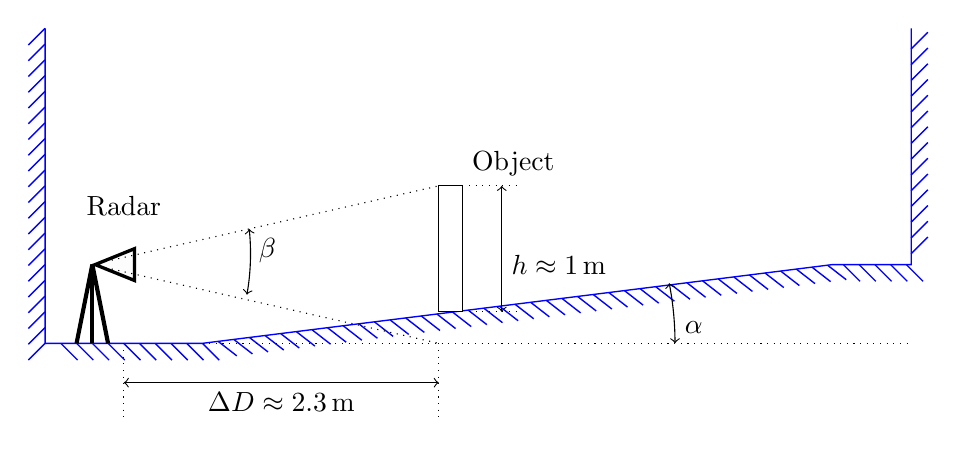
\begin{tikzpicture}[
    media/.style={font={\footnotesize\sffamily}},
    wave/.style={
        decorate,decoration={snake,post length=1.4mm,amplitude=2mm,
        segment length=2mm},thick},
    interface/.style={
        % The border decoration is a path replacing decorator.
        % For the interface style we want to draw the original path.
        % The postaction option is therefore used to ensure that the
        % border decoration is drawn *after* the original path.
        postaction={draw,decorate,decoration={border,angle=-45,
        amplitude=0.3cm,segment length=2mm}}},
    ]
        % Interface
        \draw[blue,line width=.5pt,interface] (-6, 4) -- (-6,0) -- (-4,0) -- (4,1) -- (5,1) -- (5, 4);
        % Radar
        \node[isosceles triangle, isosceles triangle apex angle=44,draw,
            inner sep=0pt,anchor=center,rotate=180,draw=black,
            line width=1.2pt, minimum height=0.5cm, fill=gray!2] (triangle) at (-5,1) {};
        \draw[black, line width=1.5pt, -] (-5.4,0) -- (-5.4,1);
        \draw[black, line width=1.5pt, -] (-5.6,0) -- (-5.4,1);
        \draw[black, line width=1.5pt, -] (-5.2,0) -- (-5.4,1);
        \filldraw[black] (-5,1.5) circle (0pt) node[above]{Radar};
        % Object
        \filldraw[fill=white,draw=black] (-1,0.4) rectangle (-0.7,2) node[above right,black]{Object};
        \draw[black,dotted] (-0.7, 2) -- (0,2);
        \draw[black,dotted] (-0.7, 0.4) -- (0,0.4);
        \draw[black,<->] (-0.2, 0.4) -- (-0.2,1) node[right]{$h \approx \SI{1}{m}$} -- (-0.2,2);

        \draw[black,<->] (2,0) node[above right] {$\alpha$} arc (0:11:4);
        \draw[black,dotted] (-4,0) -- (5,0);
        \draw[black,dotted] (-5,0) -- (-5,-1);
        \draw[black,dotted] (-1,0) -- (-1,-1);
        \draw[black, <->] (-5,-0.5) -- (-3,-0.5) node[below] {$\Delta D \approx \SI{2.3}{\meter}$} -- (-1,-0.5);

        \draw[black,dotted] (-5.4,1) -- (-1,2);
        \draw[black,dotted] (-5.4,1) -- (-1,0);
        \draw[black,<->] (-5.4,1)++(-11:2) arc (-10:6:3) node[below right] {$\beta$};

    \end{tikzpicture}
    \caption{Physical setting of the radar and objects}
    \label{fig:placement}
\end{figure}
In Figure~\ref{fig:placement} we describe the radar placement in the space.
The radar is placed opposite to a building, on a flat surface that goes into a slope of angle $\alpha$, which leads into an another building.
On the slope we place a target object of height $h$.
This object is a part of the second round of measurements.

\subsection{Internals}
\label{subsec:radar-internals}

\begin{figure}[h]
    \centering
    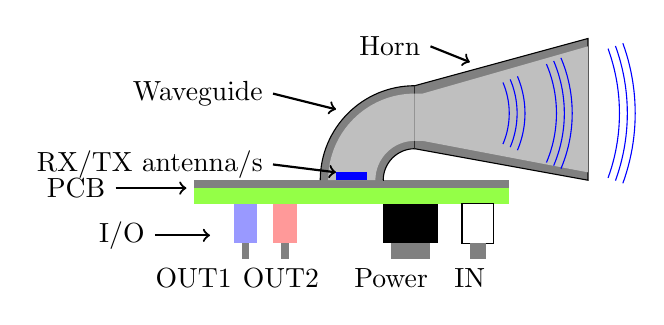
\begin{tikzpicture}
        % PCB
        \fill[green!60!white!70!yellow] (0,0) rectangle (4,0.2);
        \fill[gray] (0,0.2) rectangle (4,0.3);

        % I/O
        \fill[blue!40!white] (0.5,-0.5) rectangle (0.8,0);
        \fill[gray] (0.6,-0.7) node[below left,black]{OUT1} rectangle (0.7,-0.5);
        \fill[red!40!white] (1,-0.5) rectangle (1.3,0);
        \fill[gray] (1.1,-0.7) node[below,black]{OUT2} rectangle (1.2,-0.5);

        \fill[black] (2.4,-0.5) rectangle (3.1,0);
        \fill[gray] (2.5,-0.7) node[below,black]{Power} rectangle (3,-0.5);
        \filldraw[fill=white, draw=black] (3.4,-0.5) rectangle (3.8,0);
        \fill[gray] (3.5,-0.7) node[below,black]{IN} rectangle (3.7,-0.5);

        % Antenna
        \filldraw[fill=gray,draw=black] (1.6,0.3) arc (180:90:1.2) -- (2.8,0.7) arc (90:180:0.4) -- (2.4,0.3);
        \fill[lightgray] (1.7,0.3) arc (180:90:1.1) -- (2.8,0.8) arc (90:180:0.5) -- (2.3,0.3);
        \fill[blue] (1.8,0.3) rectangle (2.2,0.4);
        \filldraw[fill=gray,draw=black] (2.8,1.5) -- (5,2.1) -- (5,0.3) -- (2.8,0.7);
        \fill[fill=lightgray] (2.8,1.4) -- (2.9,1.4) -- (5,2) -- (5,0.4) -- (2.9,0.8) -- (2.8,0.8);

        % Radiation
        % Wave 1
        \draw [blue, xshift=3cm, yshift=1.15cm, domain=-23:23] plot(\x:1);
        \draw [blue, xshift=3cm, yshift=1.15cm, domain=-23:23] plot(\x:1.1);
        \draw [blue, xshift=3cm, yshift=1.15cm, domain=-23:23] plot(\x:1.2);
        % Wave 2
        \draw [blue, xshift=3cm, yshift=1.15cm, domain=-23:23] plot(\x:1.6);
        \draw [blue, xshift=3cm, yshift=1.15cm, domain=-23:23] plot(\x:1.7);
        \draw [blue, xshift=3cm, yshift=1.15cm, domain=-23:23] plot(\x:1.8);
        % Wave 2
        \draw [blue, xshift=3cm, yshift=1.15cm, domain=-20:20] plot(\x:2.4);
        \draw [blue, xshift=3cm, yshift=1.15cm, domain=-20:20] plot(\x:2.5);
        \draw [blue, xshift=3cm, yshift=1.15cm, domain=-20:20] plot(\x:2.6);

        % Indications
        \draw[black,thick,->] (-0.5,-0.4) node[left]{I/O} -- (0.2,-0.4);
        \draw[black,thick,->] (1,0.5) node[left]{RX/TX antenna/s} -- (1.8,0.4);
        \draw[black,thick,->] (1,1.4) node[left]{Waveguide} -- (1.8,1.2);
        \draw[black,thick,->] (3,2) node[left]{Horn} -- (3.5,1.8);
        \draw[black,thick,->] (-1,0.2) node[left]{PCB} -- (-0.1, 0.2);
    \end{tikzpicture}
    \caption{Radar schematics}
    \label{fig:radar_schematics}
\end{figure}

Figure~\ref{fig:radar_schematics} presents the approximate schematics of the radar: connections, circuit and antenna feed.
The printed circuit board (PCB) contains several elements, such as:
\begin{itemize}
    \item a power connection for signal amplification;
    \item input/output (I/O) connections, one for the signal to be emitted and 2 receiving channels, from which only the second one is used in the experiment;
    \item antennas to receive and transmit electromagnetic radiation.
\end{itemize}

The construction above the antenna is called an antenna feed.
It is used to make the design more compact, while achieving directional high density radiation.
The waveguide collects more or less unidirectional wave of the emitting element and forces it into a particular direction, in this case to the horn.

The idea of the horn is that it slowly "adapts" the wave to the space after the opening.
Otherwise a reflection can happen due to a big difference in impedance on the edge between waveguide and open air (or open space).
Thus this preserves radiation density that was achieved with the initial usage of a waveguide.

Exact circuit schemes or their components, or the name of the radar series are unknown.

\subsection{Characteristics}
\label{subsec:characteristics}

Important experiment parameters, including radar characteristics (? means unknown):
\begin{itemize}
    \item radar chirp (Fig.~\ref{fig:chirp_reflection_to_if}):
    \begin{itemize}
        \item frequency function form: sawtooth;
        \item start frequency $f_c = \SI[parse-numbers = false]{?}{\hertz}$;
        \item duration $T_c = \SI[parse-numbers = false]{?}{\second}$;
        \item bandwidth $B = \SI[parse-numbers = false]{?}{\giga\hertz}$, somewhere in millimeter band (\SI[parse-numbers = false]{30-300}{\giga\hertz});
        \item slope $S = \SI{1950037684072.2034}{\hertz\per\second}$.
    \end{itemize}
    \item number of samples $r = 3202$ over the chirp duration $T_c$;
    \item distance $\Delta D$ to the object is approximately \SI{2.3}{m};
    \item slope angle $\alpha = \SI[parse-numbers=false]{?}{\degree}$ (Fig.~\ref{fig:placement});
    \item antenna gain is unknown, including the angle of the horn radiation $\beta = \SI[parse-numbers=false]{?}{\degree}$;
    \item the object parameters:
    \begin{itemize}
        \item height $h \approx \SI{1}{m}$;
        \item consists of unknown type of plastic with unknown reflectance for millimeter waves.
    \end{itemize}
\end{itemize}


\section{Radar working principle}
\label{sec:radar-working-principle}
In this section we discuss the working principle of a frequency-modulated continuous wave (FMCW) radar that we use in the workshop.

\begin{figure}[h]
    \centering
    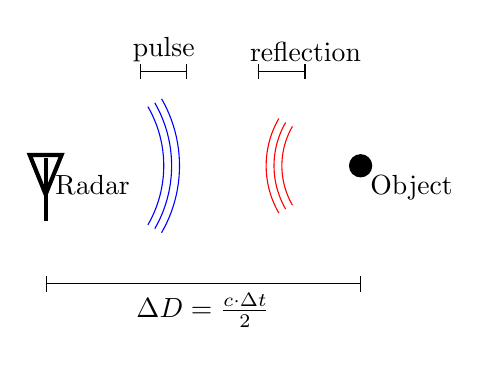
\begin{tikzpicture}
        \node[isosceles triangle, isosceles triangle apex angle=44,draw,
        inner sep=0pt,anchor=center,rotate=-90,draw=black,
        line width=1.5pt, minimum height=0.5cm, fill=gray!2] (triangle) at (0,1) {};
        \draw[black, line width=1.5pt, -] (0,0.3) -- (0,1.1);
        \filldraw[black] (0,1) circle (0pt) node[below right]{Radar};
        \filldraw[black] (4,1) circle (4pt) node[below right]{Object};

        \draw[black, |-|] (0,-0.5) -- (2,-0.5) node[below] {$\Delta D = \frac{c \cdot \Delta t}{2}$} -- (4,-0.5) ;

        \draw [blue, yshift=1cm, domain=-30:30] plot(\x:1.5);
        \draw [blue, yshift=1cm, domain=-30:30] plot(\x:1.6);
        \draw [blue, yshift=1cm, domain=-30:30] plot(\x:1.7);
        \draw[black, |-|] (1.2,2.2) -- (1.5,2.2) node[above] {pulse} -- (1.8,2.2);

        \draw [red, xshift=4cm, yshift=1cm, domain=150:210] plot(\x:1);
        \draw [red, xshift=4cm, yshift=1cm, domain=150:210] plot(\x:1.1);
        \draw [red, xshift=4cm, yshift=1cm, domain=150:210] plot(\x:1.2);
        \draw[black, |-|] (2.7,2.2) -- (3.3,2.2) node[above] {reflection};
    \end{tikzpicture}
    \caption{Radar principle overview}
    \label{fig:radar_principle}
\end{figure}

All radars operate with the same basic idea: a wave is emitted and the reflection is collected (see Fig.~\ref{fig:radar_principle}).
Then the time difference $\Delta t$ between wave emission and its reception is computed.
As the speed of light $c$ in the space we usually operate (Earth atmosphere) is known, and electromagnetic waves of any frequency always travel with this speed, it is trivial to compute the distance knowing the time difference: \[\Delta D = \frac{c \cdot \Delta t}{2}\]
Important to note, that we observe a round-trip of the wave, thus the distance obtained have to be divided by 2.

The FMCW radar have the same underlying idea, but instead of one pulse, it produces a "chirp" or a "ramp" (see Fig.~\ref{fig:chirp_amplitude}): a wave of duration $T_c$, starting with a base frequency $f_c$, which linearly increases up to frequency $f_c + B$, where $B$ is the radar bandwidth (in \SI{}{\hertz}).
The transmission chirp can be modelled by the equation $F_c(t) = S \cdot (t \mod T_c)$, where $S$ is a slope or speed of frequency change (thus $B = S \cdot T_c$).
This chirp is then reflected from an object, and appear for the receiver as a time shifted original chirp.
The reflection can be modelled as a $F_r(t) = S \cdot (t - \Delta t \mod T_c) \;\text{if}\; t \geq \Delta t \;\text{else}\; 0$, where $\Delta t$ is a time between start of a shirp and receiving it back (see Fig.~\ref{fig:chirp_reflection_to_if}).

\begin{figure}[h]
    \centering
    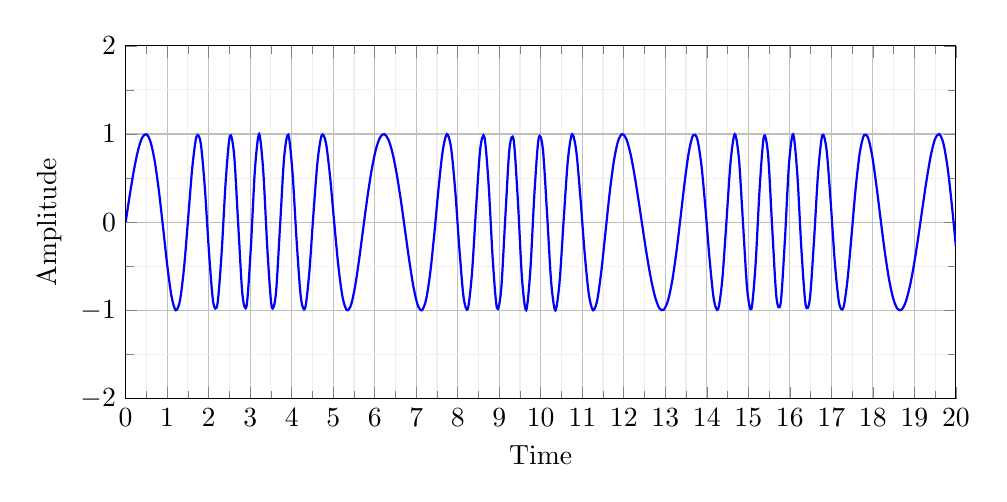
\begin{tikzpicture}
        \begin{axis}[
        xmin = 0, xmax = 20,
        ymin = -2, ymax = 2,
        xtick distance = 1,
        ytick distance = 1,
        grid = both,
        minor tick num = 1,
        major grid style = {lightgray},
        minor grid style = {lightgray!25},
        width = \textwidth,
        height = 0.5\textwidth,
        xlabel = {Time},
        ylabel = {Amplitude},]
        \addplot[
            domain = 0:20,
            samples = 200,
            smooth,
            thick,
            blue,
        ] {sin(deg(pi*(2*x-sin(deg(x))) + 2*pi))};
        \end{axis}
    \end{tikzpicture}
    \caption{Chirp example (sinusoidal frequency change)}
    \label{fig:chirp_amplitude}
\end{figure}

\begin{figure}[h]
    \centering
    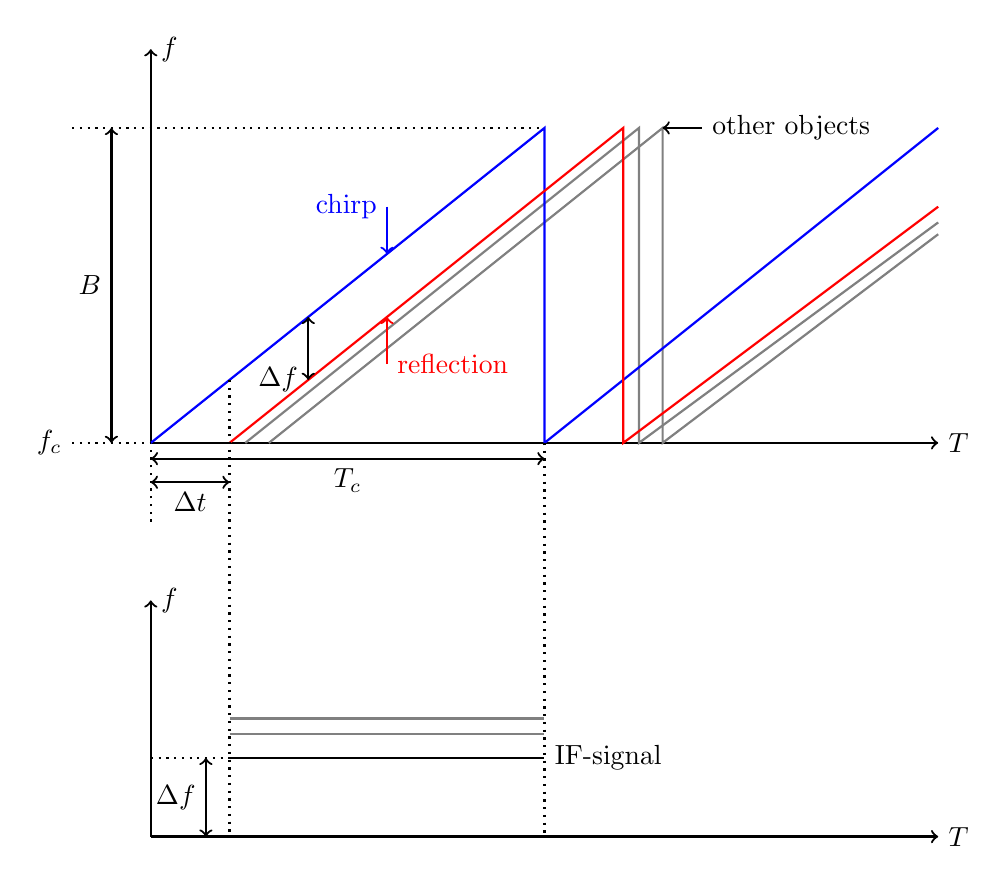
\begin{tikzpicture}
        % T (x)
        \draw[black, thick, ->] (0,0) -- (10,0) node[right] {$T$};
        % f (y)
        \draw[black, thick, ->] (0,0) -- (0,5) node[right] {$f$};
        \draw[black, thick, dotted] (0,-1) -- (0,0);

        % secondary reflections
        \draw[gray, thick, -] (1.2,0) -- (6.2,4) -- (6.2,0) -- (10,2.8);
        \draw[gray, thick, -] (1.5,0) -- (6.5,4) -- (6.5,0) -- (10,2.65);
        % chirp
        \draw[blue, thick, -] (0,0) -- (5,4) -- (5,0) -- (10,4);
        % primary reflection
        \draw[red, thick, -] (1,0) -- (6,4) -- (6,0) -- (10,3);

        \draw[black, thick, <->] (2,4/5) node[left] {$\Delta f$} -- (2,2*4/5);
        \draw[black, thick, <->] (0, -0.5) -- (0.5,-0.5) node[below] {$\Delta t$} -- (1,-0.5);
        \draw[black, thick, <->] (0, -0.2) -- (2.5,-0.2) node[below] {$T_c$} -- (5,-0.2);

        \draw[blue, thick, ->]  (3,3) node[left] {chirp} -- (3,3*4/5);
        \draw[red, thick, ->]  (3,1) node[right] {reflection} -- (3,2*4/5);
        \draw[black, thick, ->]  (7,4) node[right] {other objects} -- (6.5,4);

        \draw[black, thick, dotted] (-1,0) node[left] {$f_c$}-- (0,0);
        \draw[black, thick, dotted] (-1,4) -- (5,4);
        \draw[black, thick, <->] (-0.5,0) -- (-0.5,2) node[left]{$B$} -- (-0.5,4);

        % T (x)
        \draw[black, thick, ->] (0,-5) -- (10,-5) node[right] {$T$};
        % f (y)
        \draw[black, thick, ->] (0,-5) -- (0,-2) node[right] {$f$};

        \draw[gray, thick, -] (1,-3.5) -- (5,-3.5);
        \draw[gray, thick, -] (1,-3.7) -- (5,-3.7);
        \draw[black, thick, -] (1,-4) -- (5,-4) node[right] {IF-signal};
        \draw[black, thick, <->] (0.7,-5) -- (0.7, -4.5) node[left] {$\Delta f$} -- (0.7,-4);
        \draw[black, thick, dotted] (0,-4) -- (1,-4);
        \draw[black, thick, dotted] (1,4/5) -- (1,-5);
        \draw[black, thick, dotted] (5,0) -- (5,-5);
    \end{tikzpicture}
    \caption{Chirp, reflections and IF-signal frequency tones.}
    \label{fig:chirp_reflection_to_if}
\end{figure}

So, in a radar we observe these 2 functions at the same time, but in the end we need $\Delta t$.
We can find it by subtraction:
\[F_c(t) - F_r(t) = S \cdot t - S \cdot (t - \Delta t) = S \cdot \Delta t\]

Thus in the radar we put a component, called mixer, that outputs $\Delta f = f_t - f_r$, which is the instantaneous difference of transmitted and received waves' frequencies.
We use it as a substritute for $F_c(t) - F_r(t)$ part, from which roundtrip time is trivial to obtain via an equation $\Delta t = \frac{\Delta f}{S}\SI{}{s}$.
And from this roundtrip time, the distance can be obtained: $\Delta D = \frac{c \cdot \Delta t}{2}$.
Or as a complete equation: \[\Delta D = \frac{\Delta f \cdot c}{2S}\SI{}{m}\]

If there are several objects, there would be several waves mixed together (see Fig.~\ref{fig:if_signal}, an amplitude-time version of second part of Fig.~\ref{fig:chirp_reflection_to_if}), which will arrive at the same time to the radar.
As they differ in the distance, the shift is different for all of them, and thus the frequency difference.
The mixed signal received is called IF-signal or beat, and by using the Fast Fourier Transform (FFT), we can distinguish their corresponding frequencies in it (Fig.~\ref{fig:fft_frequencies} shows frequency components of the wave from Fig.~\ref{fig:if_signal}) and thus the distances.

\begin{figure}[h]
    \centering
    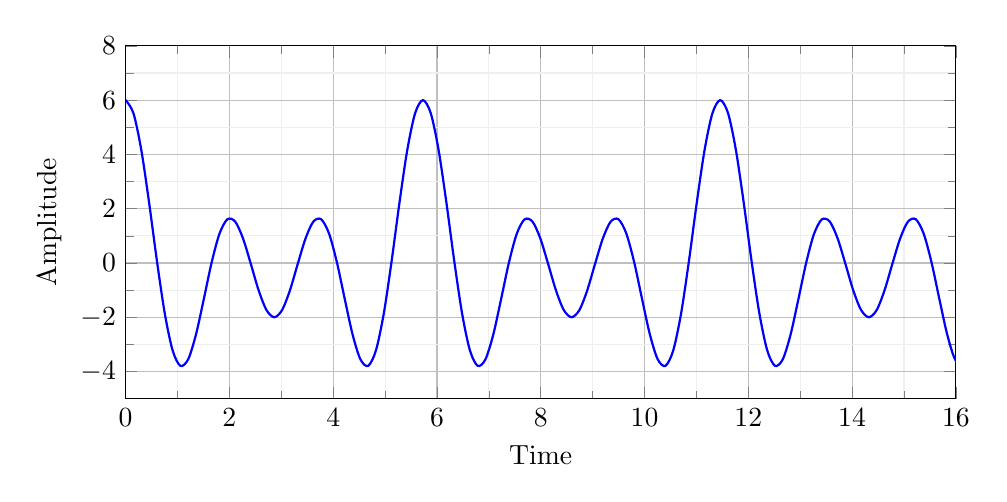
\begin{tikzpicture}
        \begin{axis}[
        xmin = 0, xmax = 16,
        ymin = -5, ymax = 8,
        xtick distance = 2,
        ytick distance = 2,
        grid = both,
        minor tick num = 1,
        major grid style = {lightgray},
        minor grid style = {lightgray!25},
        width = \textwidth,
        height = 0.5\textwidth,
        xlabel = {Time},
        ylabel = {Amplitude},]
        \addplot[
            domain = 0:30,
            samples = 200,
            smooth,
            thick,
            blue,
        ] {cos(20*pi*x) + 2*cos(2*20*pi*x) + 3*cos(3*20*pi*x)};
        \end{axis}
    \end{tikzpicture}
    \caption{Example IF-signal}
    \label{fig:if_signal}
\end{figure}

\begin{figure}[h]
    \centering
    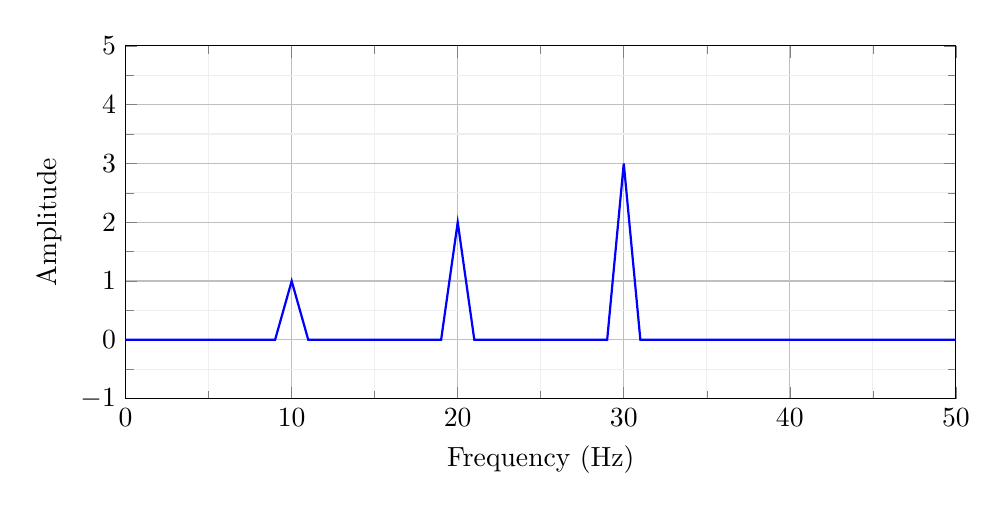
\begin{tikzpicture}
        \begin{axis}[
        xmin = 0, xmax = 50,
        ymin = -1, ymax = 5,
        xtick distance = 10,
        ytick distance = 1,
        grid = both,
        minor tick num = 1,
        major grid style = {lightgray},
        minor grid style = {lightgray!25},
        width = \textwidth,
        height = 0.5\textwidth,
        xlabel = {Frequency (Hz)},
        ylabel = {Amplitude},]
        \addplot[
            thick,
            blue,
        ]
        coordinates {
            (0,0)(9,0)(10,1)(11,0)(19,0)(20,2)(21,0)(29,0)(30,3)(31,0)(50,0)
        };
        \end{axis}
    \end{tikzpicture}
    \caption{Frequency spectrum of the IF-signal}
    \label{fig:fft_frequencies}
\end{figure}

The complete procedure for the distance measurement of FMCW radar is:
\begin{enumerate}
    \item start modulation;
    \item record IF-signal for a $T_c$ window;
    \item perform FFT;
    \item scale obtained FFT frequencies axis with $\frac{c}{2S}$;
    \item the result is a dataset with $x$ axis being distance and $y$ being the strength of reflection at this distance;
    \item the anomalous spikes indicate higher reflection in the space at the calculated distance, and thus objects.
\end{enumerate}

\section{Data processing}
\label{sec:data-post-processing}
Input data of the experiment are 2 sets of 16 vectors of If-signal measurements, each of size 3202.
One set contains measurements without the object of interest, and the second one is with the object.

We perform the same procedure described as in the Section.~\ref{sec:radar-working-principle}, with a difference, that we:
\begin{enumerate}
    \item average 16 measurements to minimize clutter (random noice caused by environment with non-ideal density distribution, which reflects the waves back, even from air);
    \item calculate difference between results of measurements without object with the results with object, in order to remove the environment and highlight the object.
\end{enumerate}

The procedure is implemented in both Rust and Python.
The source code is open and available in the following repository: \url{https://github.com/PaulRaUnite/scientific_course}.

Considering placement described in Fig.~\ref{fig:placement}, we should expect a spike at around \SI{2.3}{m}, with some other objects that we couldn't control in the real experiment (birds, passing people, etc), i.e something similar to Fig.~\ref{fig:experiment_expectation}.\footnote{The amplitude is assigned arbitrarily.}
This does correspond to the result of the experiment (Fig.~\ref{fig:experiment_reality}), where we see a spike around \SI{2.3}{m}.

\begin{figure}[h]
    \centering
    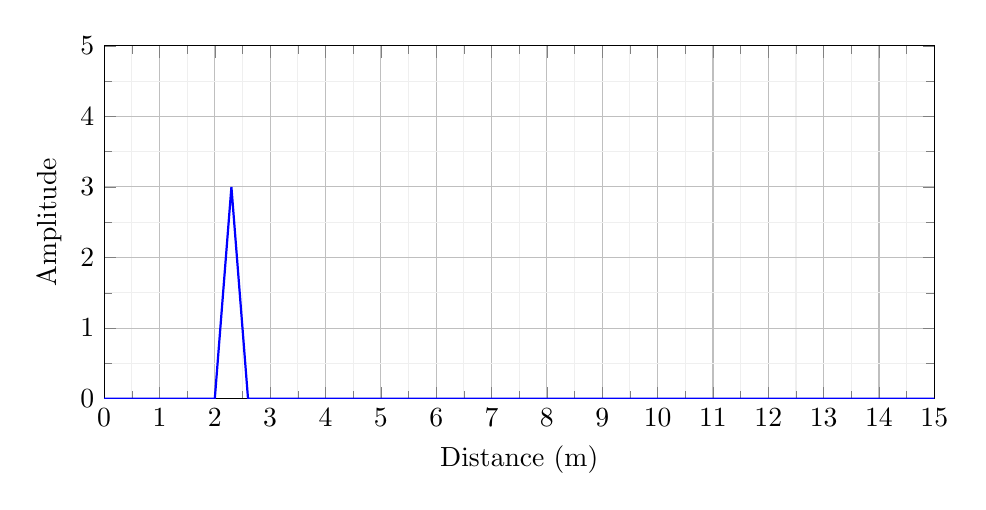
\begin{tikzpicture}
        \begin{axis}[
        xmin = 0, xmax = 15,
        ymin = 0, ymax = 5,
        xtick distance = 1,
        ytick distance = 1,
        grid = both,
        minor tick num = 1,
        major grid style = {lightgray},
        minor grid style = {lightgray!25},
        width = \textwidth,
        height = 0.5\textwidth,
        xlabel = {Distance (m)},
        ylabel = {Amplitude},]
            \addplot[
                thick,
                blue,
            ]
            coordinates {
                (0,0)(2,0)(2.3,3)(2.6,0)(15,0)
            };
        \end{axis}
    \end{tikzpicture}
    \caption{Expected distance data of the experiment}
    \label{fig:experiment_expectation}
\end{figure}

\begin{figure}[h]
    \centering
    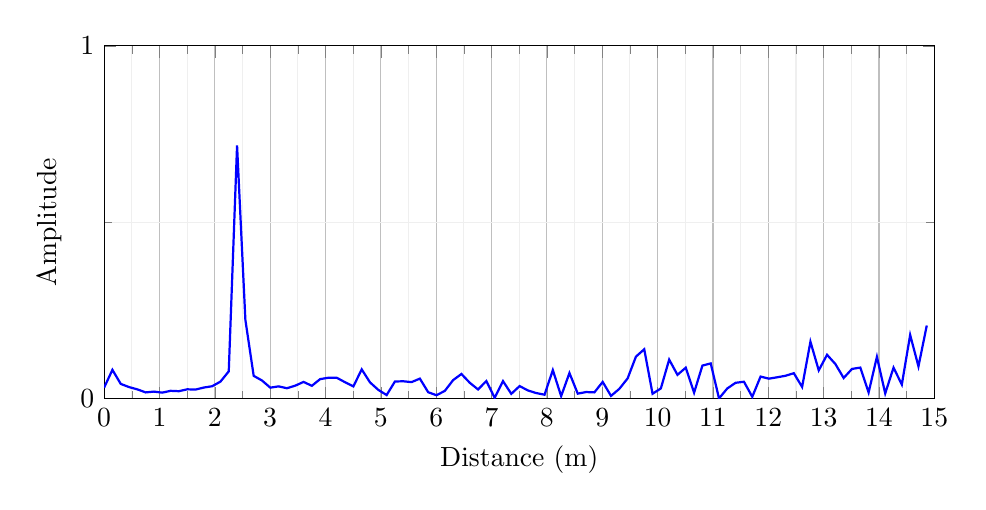
\begin{tikzpicture}
        \begin{axis}[
        xmin = 0, xmax = 15,
        ymin = 0, ymax = 1,
        xtick distance = 1,
        ytick distance = 1,
        grid = both,
        minor tick num = 1,
        major grid style = {lightgray},
        minor grid style = {lightgray!25},
        width = \textwidth,
        height = 0.5\textwidth,
        xlabel = {Distance (m)},
        ylabel = {Amplitude},]
        \addplot[
            thick,
            blue,
        ]
        coordinates {
            (0.0,0.03124502182680544)(0.15013354596012252,0.08165254160493873)(0.30026709192024503,0.04187154002650573)(0.45040063788036755,0.03279359417989269)(0.6005341838404901,0.026346019557180966)(0.7506677298006126,0.017735071416026926)(0.9008012757607351,0.01998810137331475)(1.0509348217208576,0.01708494864236343)(1.2010683676809801,0.02219449458468148)(1.3512019136411026,0.021146432503272194)(1.5013354596012252,0.026497042294707285)(1.6514690055613477,0.02572798031161483)(1.8016025515214702,0.0315015968395187)(1.9517360974815927,0.03519442458279798)(2.1018696434417152,0.048264513082713734)(2.2520031894018375,0.07730853473293564)(2.4021367353619603,0.7174413976132712)(2.5522702813220826,0.223362314550144)(2.7024038272822053,0.06464055671958135)(2.8525373732423276,0.05149268566681542)(3.0026709192024503,0.031163588893889482)(3.1528044651625726,0.03483832320073077)(3.3029380111226954,0.02954330436504904)(3.4530715570828177,0.03681031660636336)(3.6032051030429404,0.04742717185852996)(3.7533386490030627,0.03643438749857353)(3.9034721949631854,0.05542695950877885)(4.053605740923308,0.059274703161747766)(4.2037392868834305,0.05919027455301773)(4.353872832843552,0.0465220459317095)(4.504006378803675,0.03487725178572987)(4.654139924763798,0.08293836302699731)(4.8042734707239205,0.046076080752598614)(4.954407016684042,0.024854320507031957)(5.104540562644165,0.010238338579796391)(5.254674108604288,0.04869034931323313)(5.404807654564411,0.04922458478594649)(5.554941200524532,0.046935872918709265)(5.705074746484655,0.0568027356818277)(5.855208292444778,0.01826204452829927)(6.005341838404901,0.009707268991775209)(6.1554753843650225,0.02200619509537205)(6.305608930325145,0.052502597043798005)(6.455742476285268,0.06997048763034286)(6.605876022245391,0.04512123442057714)(6.756009568205513,0.026130092606109656)(6.906143114165635,0.049978008759708814)(7.056276660125758,0.0022665466073448215)(7.206410206085881,0.049869379754852616)(7.356543752046003,0.01364059868694767)(7.506677298006125,0.03566540889794112)(7.656810843966248,0.023306440032811793)(7.806944389926371,0.01586774791169887)(7.957077935886493,0.011164221292716547)(8.107211481846615,0.08093406297716399)(8.257345027806737,0.007184675480999658)(8.407478573766861,0.07263314259944309)(8.557612119726983,0.014222416305059937)(8.707745665687105,0.018744071468830725)(8.857879211647228,0.01777627911579316)(9.00801275760735,0.047454885301419836)(9.158146303567474,0.007809426421417243)(9.308279849527596,0.02771907040639121)(9.458413395487717,0.05743828749950808)(9.608546941447841,0.11907748438162002)(9.758680487407963,0.14001965316744247)(9.908814033368085,0.01389992726599587)(10.058947579328208,0.02900066828499348)(10.20908112528833,0.11071237224469144)(10.359214671248454,0.06755081697573928)(10.509348217208576,0.08788942572859071)(10.659481763168698,0.017055473513522657)(10.809615309128821,0.0936908861198873)(10.959748855088943,0.09988724719822528)(11.109882401049065,0.0006609848642398219)(11.260015947009189,0.029145099042750644)(11.41014949296931,0.044953956451195154)(11.560283038929434,0.0479585520827186)(11.710416584889556,0.0053408856714440844)(11.860550130849678,0.0626039916336083)(12.010683676809801,0.056645844401074896)(12.160817222769923,0.06055882624626463)(12.310950768730045,0.06487409875231265)(12.461084314690169,0.07214206011524027)(12.61121786065029,0.03324333689913317)(12.761351406610412,0.16139949381417296)(12.911484952570536,0.08025097604480891)(13.061618498530658,0.12432821936219796)(13.211752044490781,0.09823422263545467)(13.361885590450903,0.05854760009104609)(13.512019136411025,0.08424084198614423)(13.662152682371149,0.08806448589545823)(13.81228622833127,0.017344332696993092)(13.962419774291392,0.11851834098942504)(14.112553320251516,0.014868218924391385)(14.262686866211638,0.08783555901548823)(14.412820412171762,0.03993753330733796)(14.562953958131883,0.18064987093029572)(14.713087504092005,0.0914160956196639)(14.863221050052129,0.20720923425518833)

        };
        \end{axis}
    \end{tikzpicture}
    \caption{Actual distance data of the experiment}
    \label{fig:experiment_reality}
\end{figure}

\section{Criticism}\label{sec:criticism}
There are several factors that influence the precision, cleanness and reproducibility of the experiment.
These include:
\begin{enumerate}
%    \item the experiment is conducted on open air, the precise parameters of which are not known (the speed of light and impedance);
    \item some of the parameters of the radar are unknown ($f_c, T_c, B,\beta$) and cannot be inferred from the experiment itself or other parameters, which makes the experiment harder to reproduce;
    \item the object is placed on the slope, which adds noice to the input, possibly in a pattern that can show up as an additional object or smear the target object;
    \item environment is not fully controlled, and external bodies can enter the area of the experiment freely, sabotaging the results.
\end{enumerate}

\section{Conclusion}\label{sec:conclusion}
FMCW radar is a powerful tool that is able to measure distances precisely up to resolution $d_{res} = \frac{c}{2B}$, and to determine a relative speed of the object using the Doppler effect (which is not covered by the workshop).
In this workshop we briefly covered the theoretical aspect of its working and we were able to produce code that calculates object distances with the results that match the expected behaviour.

%\bibliography{refs}
%\bibliographystyle{plain}
\end{document}